\section{Peer-to-Peer and Federated Adapter Learning}
\label{sec:p2p_federated}

\noindent\textbf{SQ5:} \textit{What decentralised infrastructure and protocols
exist for adapter-level exchange without a central coordinating server?} This
section surveys both bodies of work, making explicit what each contributes
and what it leaves open; SQ5 is resolved in the centralised discussion in
Section~\ref{sec:synthesis_gap:answers}.

\subsection{Federated Learning Foundations}
\label{sec:p2p_federated:fl_foundations}

McMahan et al.~\cite{McMahan2017} introduced Federated Averaging (FedAvg), the foundational algorithm
for learning from decentralised data without moving raw data to a central server. In
FedAvg, a central server distributes the current global model to a subset of participating
clients; each client performs several steps of local stochastic gradient descent on its
private data; the resulting local model updates are communicated back to the server and
averaged to produce the next global model. By exchanging model weights rather than raw
gradients or data, FedAvg reduces communication cost by one to two orders of magnitude
compared to synchronous distributed SGD, while preserving data locality.

The primary challenge for FedAvg in heterogeneous deployments is the \textit{non-IID}
problem: when client data distributions diverge, client updates point in contradictory
directions, and naive averaging degrades towards a global model that performs poorly
on any individual client's distribution. Li et al.~\cite{Li2020FedProx} proposed FedProx, which
adds a proximal regularisation term to the client objective:

\begin{equation}
\min_{w_k} \; h_k(w_k) + \frac{\mu}{2} \|w_k - w\|^2
\label{eq:fedprox}
\end{equation}

where $h_k$ is client $k$'s local loss, $w$ is the current global model, and $\mu > 0$
controls the strength of the pull towards the global model. The proximal term bounds
local drift under data heterogeneity, enabling convergence even when clients complete
different numbers of local update steps (partial work). FedProx consistently outperforms
FedAvg on non-IID benchmarks by 1--5 percentage points in test accuracy and is the
reference baseline for heterogeneity-tolerant federated optimisation \cite{Li2020FedProx}.

\subsection{Gossip Learning and Decentralised FL}
\label{sec:p2p_federated:gossip}

FedProx improves on FedAvg but retains two limitations: (i)~it assumes all participating nodes use 
a uniform model architecture (homogeneous model assumption); and (ii)~the central server remains 
a single point of failure even though client updates are more stable under heterogeneity. 
The first limitation is particularly relevant to the decentralised setting examined in this review, 
since a P2P exchange architecture would allow heterogeneous adapter ranks and architectures, a peer with a bottleneck adapter and one with a LoRA adapter could exchange capabilities without homogenising. 
The second limitation motivates the fully decentralised protocols discussed in the gap analysis (Section~\ref{sec:synthesis_gap}).

The centralised FL server in FedAvg and FedProx represents a single point of failure and
a coordination bottleneck. The gossip learning literature removes this dependency by
having peers communicate directly with randomly selected neighbours. In gossip learning,
each node periodically samples a peer, exchanges model parameters with that peer, and
averages the received parameters with its own local model \cite{OrmandyGossip2013}.

Heged{\H{u}}s et al.~\cite{HegeduisGossip2019} demonstrated that gossip learning matches or outperforms
FL quality in simulation while eliminating the central aggregator. Convergence is
faster than FL per communication round due to the direct peer-to-peer exchange,
and the approach scales to large peer populations without
requiring any central infrastructure. Adaptive peer selection: preferring neighbours
with high estimated bandwidth or diverse data distributions improves convergence
speed in heterogeneous networks.

Fully decentralised FL without a server was formalised by Vanhaesebrouck et al.~\cite{VanhaesebrouckDCL2017},
who analysed the convergence of gossip-based averaging for convex objectives, and by
Jiang et al.~\cite{JiangCollab2017}, who proposed collaborative deep learning over a peer network
with fixed communication topology. These works established that fully decentralised
model averaging converges to the same stationary points as centralised FL under mild
conditions on graph connectivity, providing the theoretical foundation for applying
gossip-style aggregation to adapter weight matrices.

\begin{figure}[H]
  \centering
  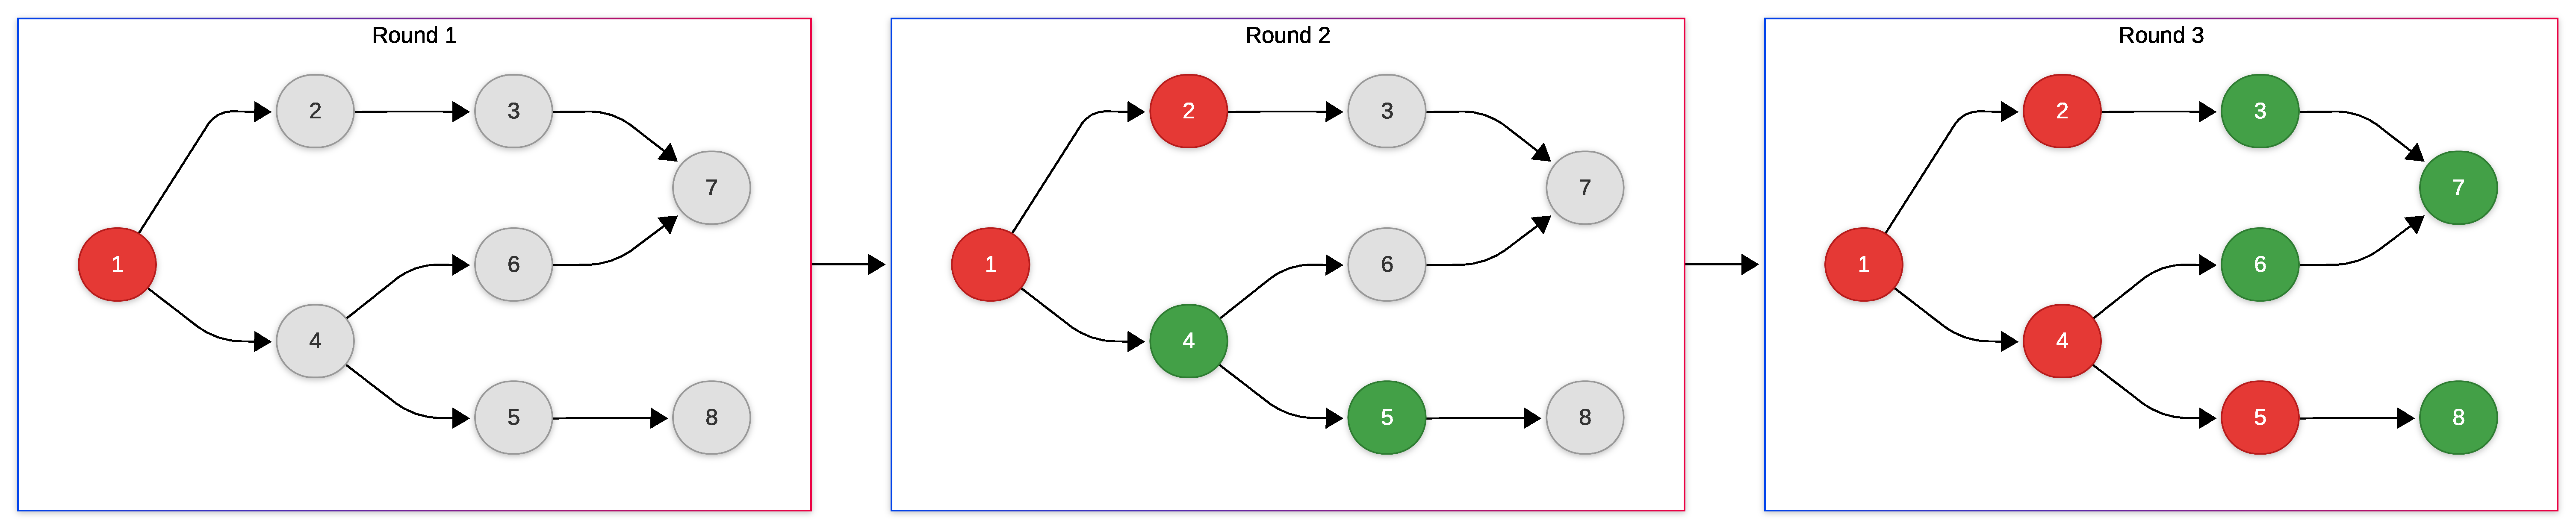
\includegraphics[width=0.75\linewidth]{figures/fig_p2p_gossip.pdf}
  \caption{Gossip learning (own figure): each node periodically samples a
    random peer, exchanges model parameters, and averages the received weights
    with its own local model. The process eliminates the central aggregator
    while maintaining convergence to the same stationary points as centralised
    FL under mild graph-connectivity conditions \cite{HegeduisGossip2019}.}
  \label{fig:gossip}
\end{figure}

\subsection{P2P Systems for Deep Learning}
\label{sec:p2p_federated:p2p_dl}

Beyond gossip learning, the P2P machine learning literature has addressed coordination
of training and inference across nodes without any fixed topology or central authority.
Bellavista et al.~\cite{BellavistaDL2021} provided a systematic review of decentralised deep learning
approaches on resource-constrained devices, classifying systems by communication
topology (ring, mesh, gossip), aggregation strategy, and fault tolerance. Wink et al.~\cite{WinkP2PFL2021}
proposed a fully P2P federated learning system without any central server, demonstrating
competitive accuracy on image classification tasks under peer churn. Ye et al.~\cite{YeDecentralizedFL2022}
extended decentralised FL to unreliable network conditions, introducing
\textit{asynchronous} gossip aggregation that maintains convergence under irregular
peer availability.

Savazzi et al.~\cite{Savazzi2020} addressed bandwidth-heterogeneous wireless P2P networks, proposing
energy-aware model aggregation policies that adapt the communication pattern to link
quality.

\subsection{P2P Transformer Inference and the MT-EF Architecture}
\label{sec:p2p_federated:p2p_transformer}

The most directly relevant P2P works for this review operate at the transformer level.
{\v{S}}ajina~\cite{Sajina2021} described the first system for multi-task P2P learning with
transformer-based models, proposing an architecture in which peers collaboratively
train and serve task-specific modules over a shared encoder backbone. {\v{S}}ajina et al.~\cite{Sajina2024}
extended this framework in a peer-to-peer multi-task environment for transformer NLP
using encoder-only models, demonstrating that multi-task performance can be maintained
while distributing task-specific computation across independent network nodes. The
{\v{S}}ajina et al.~\cite{SajinaP2PConnection2024} survey catalogued autonomous connection establishment
methods for P2P deep learning networks, identifying the lack of adapter-level discovery
protocols as an open research gap.

Borzunov et al.~\cite{Borzunov2023} introduced Petals, which applies P2P principles to LLM inference
at the layer level: volunteer nodes each host a subset of transformer layers, and
inference requests are routed through the volunteer network by passing activations
from node to node. Petals demonstrated that collaborative inference of BLOOM-176B-scale
models is feasible using commodity hardware, with practical throughput sufficient for
interactive use despite internet-scale latency. Critically, Petals does not incorporate
per-task adapter modules: all nodes serve identical shared backbone layers without task
specialisation, leaving the adapter dimension of P2P inference unexplored.
\begin{figure}[H]
  \centering
  % CREATE AN ORIGINAL FIGURE here (own drawing, no reproduction permission
  % needed): a schematic of Petals-style collaborative inference. Drop your
  % PDF into figures/ and replace the \fbox placeholder below with
  % \includegraphics.
  \fbox{\parbox{0.7\textwidth}{\centering\vspace{1.8cm}
    \textit{Figure: Petals collaborative inference architecture}\\[0.4em]
    \small(create original figure here)\vspace{1.8cm}}}
  \caption{Petals collaborative inference (own figure): volunteer nodes each
    host a contiguous subset of transformer layers; client requests are routed
    through the volunteer network by passing activations node-to-node
    \cite{Borzunov2023}. Critically, no per-task adapter modules are
    loaded---leaving the adapter dimension of P2P inference unexplored.}
  \label{fig:petals}
\end{figure}


\subsection{Federated PEFT: Integrating Adapters with Federated Learning}
\label{sec:p2p_federated:fed_peft}

The observation that PEFT adapters are dramatically smaller than full model weights
makes them well-suited units for federated communication: exchanging only the adapter
matrices reduces per-round communication by 90--99\% compared to exchanging full model
gradients or weights \cite{ZhangFedPETuning2023}. This insight motivated a substantial
body of work on federated PEFT, which applies FL algorithms to the training and
aggregation of adapter modules across distributed clients.

\paragraph{Federated adapter aggregation.}
Zhang et al.~\cite{ZhangFedPETuning2023} conducted the first systematic study of federated PEFT
(FedPETuning), evaluating LoRA, prefix tuning, and bottleneck adapters integrated with
FedAvg across non-IID partitions of text classification benchmarks. Adapters and LoRA
consistently outperformed prefix tuning under federated conditions, and adapter-only
exchange achieved over 90\% communication savings at within-5\% accuracy degradation
relative to centralised PEFT. Trautmann et al.~\cite{TrautmannAgg2024} studied the aggregation of LoRA
adapters with heterogeneous ranks, demonstrating that rank-aligned averaging maintains
near-centralised performance. Singhal et al.~\cite{SinghalFedEx2025} proposed FedEx-LoRA, an exact
aggregation method for federated LoRA that eliminates the approximation error in
standard FedAvg averaging of low-rank factors by aggregating the full product
$\Delta W = BA$ rather than the individual factor matrices.

\paragraph{Heterogeneous client resources.}
A recurring challenge in federated PEFT is that clients differ in compute capacity,
memory, and available bandwidth. Wang et al.~\cite{WangFLoRA2024} proposed FLoRA, which maintains
a global LoRA of maximum rank on the server and allows each client to fine-tune a
truncated LoRA matrix of its resource-determined rank; rank-alignment padding enables
FedAvg aggregation across heterogeneous ranks. Cho et al.~\cite{ChoHeteroLoRA2024} introduced a
heterogeneous LoRA assignment policy that allocates higher ranks to clients with larger
data or compute budgets, improving the global model quality under device heterogeneity.
Wang et al.~\cite{WangGlobecom2024} addressed the wireless channel constraints of federated
LoRA over mobile networks, showing that bandwidth-aware rank selection reduces
communication delay without degrading convergence. Gao et al.~\cite{GaoINFOCOM2025} proposed
adaptive quantization of federated LoRA weights for heterogeneous devices, enabling
clients with limited hardware to participate in aggregation by transmitting compressed
adapter updates.

\paragraph{Privacy and differential privacy.}
Liu et al.~\cite{LiuDP2023} introduced differential privacy mechanisms for federated adapter
training, adding calibrated Gaussian noise to adapter updates before transmission to
provide formal $(\epsilon, \delta)$-DP guarantees per round. Sun et al.~\cite{SunImprovingLoRA2024}
analysed the privacy--utility tradeoff for federated LoRA, demonstrating that low-rank
adapters require smaller noise magnitude than full gradients to achieve the same
privacy budget, due to their reduced dimensionality. Xu et al.~\cite{XuDPFedLoRA2025} proposed
DP-FedLoRA, an end-to-end framework combining per-sample gradient clipping with
low-rank adapter exchange, achieving formal DP guarantees with competitive accuracy
on clinical NLP benchmarks.

\paragraph{Privacy-preserving split learning.}
Lin et al.~\cite{LinSplitLoRA2024} combined split learning with LoRA fine-tuning: the transformer
stack is partitioned between the client (bottom layers) and the server (top layers), with
only the split-point activation tensor transmitted. LoRA adapters are trained on the
server-side layers, and only the adapter matrices are returned to the client after
training. This approach reduces client-side compute and communication while preserving
data privacy, at the cost of requiring a semi-trusted server. Zhang et al.~\cite{ZhangPrivacySplit2023}
extended split learning to privacy-sensitive NLP with adapter-based bottleneck compression,
reducing the mutual information between transmitted activations and raw input data.

\paragraph{Personalisation and selective aggregation.}
Cai et al.~\cite{CaiFedAdapter2023} proposed FedAdapter, combining adapter-based personalisation
with FL: a shared backbone adapter is trained globally, while a thin personalisation
head adapter is trained locally on each client's private data. This two-level
decomposition enables global task knowledge to be shared without homogenising
client-specific behaviour. Guo et al.~\cite{GuoSelective2025} introduced selective aggregation,
in which only adapter components with high cross-client agreement are included in the
global average, filtering out idiosyncratic updates that arise from client-specific
data artefacts. Yan et al.~\cite{YanFeDeRA2024} proposed FeDeRA, which performs efficient
federated adaptation by restricting updates to the singular vectors of pre-trained
weight matrices with largest variance, further reducing the dimension of the exchanged
adapter.

\paragraph{Advanced federated adapter protocols.}
Bian et al.~\cite{BianFedALT2025} proposed FedALT, which adapts the local training schedule
adaptively to the current round's data distribution signal, improving convergence
under time-varying non-IID conditions. Babakniya et al.~\cite{Babakniya2023} introduced SLoRA,
a federated variant of LoRA that initialises adapter matrices via SVD of the
accumulated gradient to align the initial low-rank subspace with the true gradient
direction, accelerating federated convergence. Zhao et al.~\cite{ZhaoFedMCP2024} proposed
FedMCP, which adds model-contrastive personalisation to federated adapter training,
pulling the client adapter towards the global model while pushing it away from
representations of other clients' data distributions to sharpen personalisation.
Liu et al.~\cite{LiuAdaptive2024} and Koo et al.~\cite{KooBai2025} addressed federated PEFT under
heterogeneous task distributions, where different clients fine-tune for entirely
different downstream tasks, demonstrating that global adapter aggregation remains
beneficial as a pretraining signal even when tasks are non-overlapping.

\subsection{DHT-Based Infrastructure for P2P Adapter Discovery}
\label{sec:p2p_federated:dht}

All of the federated systems reviewed above rely on a central aggregation server for
adapter collection and redistribution. The P2P literature provides infrastructure
primitives for performing this coordination without a central node. Maymounkov and Mazi{\`{e}}res~\cite{MaymounkovKademlia2002}
introduced the Kademlia distributed hash table (DHT), which provides $O(\log N)$
lookup of key-value pairs across a network of $N$ nodes using a XOR-distance metric.
Kademlia has been deployed at scale in BitTorrent and other P2P systems, and its
correctness and resistance to churn are well understood.

% [PROPOSED C1 - Vanja review before removing this marker]
Chord~\cite{StoicaChord2001} and BitTorrent~\cite{CohenBitTorrent2003} are foundational P2P precedents that predate Kademlia: Chord established $O(\log N)$ consistent-hashing-based lookup, and BitTorrent demonstrated at internet scale that a tit-for-tat incentive scheme can sustain robust peer cooperation without central coordination.
% [END PROPOSED C1]

Recent work on decentralised LoRA, such as Dec-LoRA by Ghiasvand et al.~\cite{Ghiasvand2025}, demonstrates that parameter-efficient LLM fine‑tuning can be performed without a central server over decentralised communication topologies, motivating similar designs for adapter-based systems.

\begin{figure}[H]
  \centering
  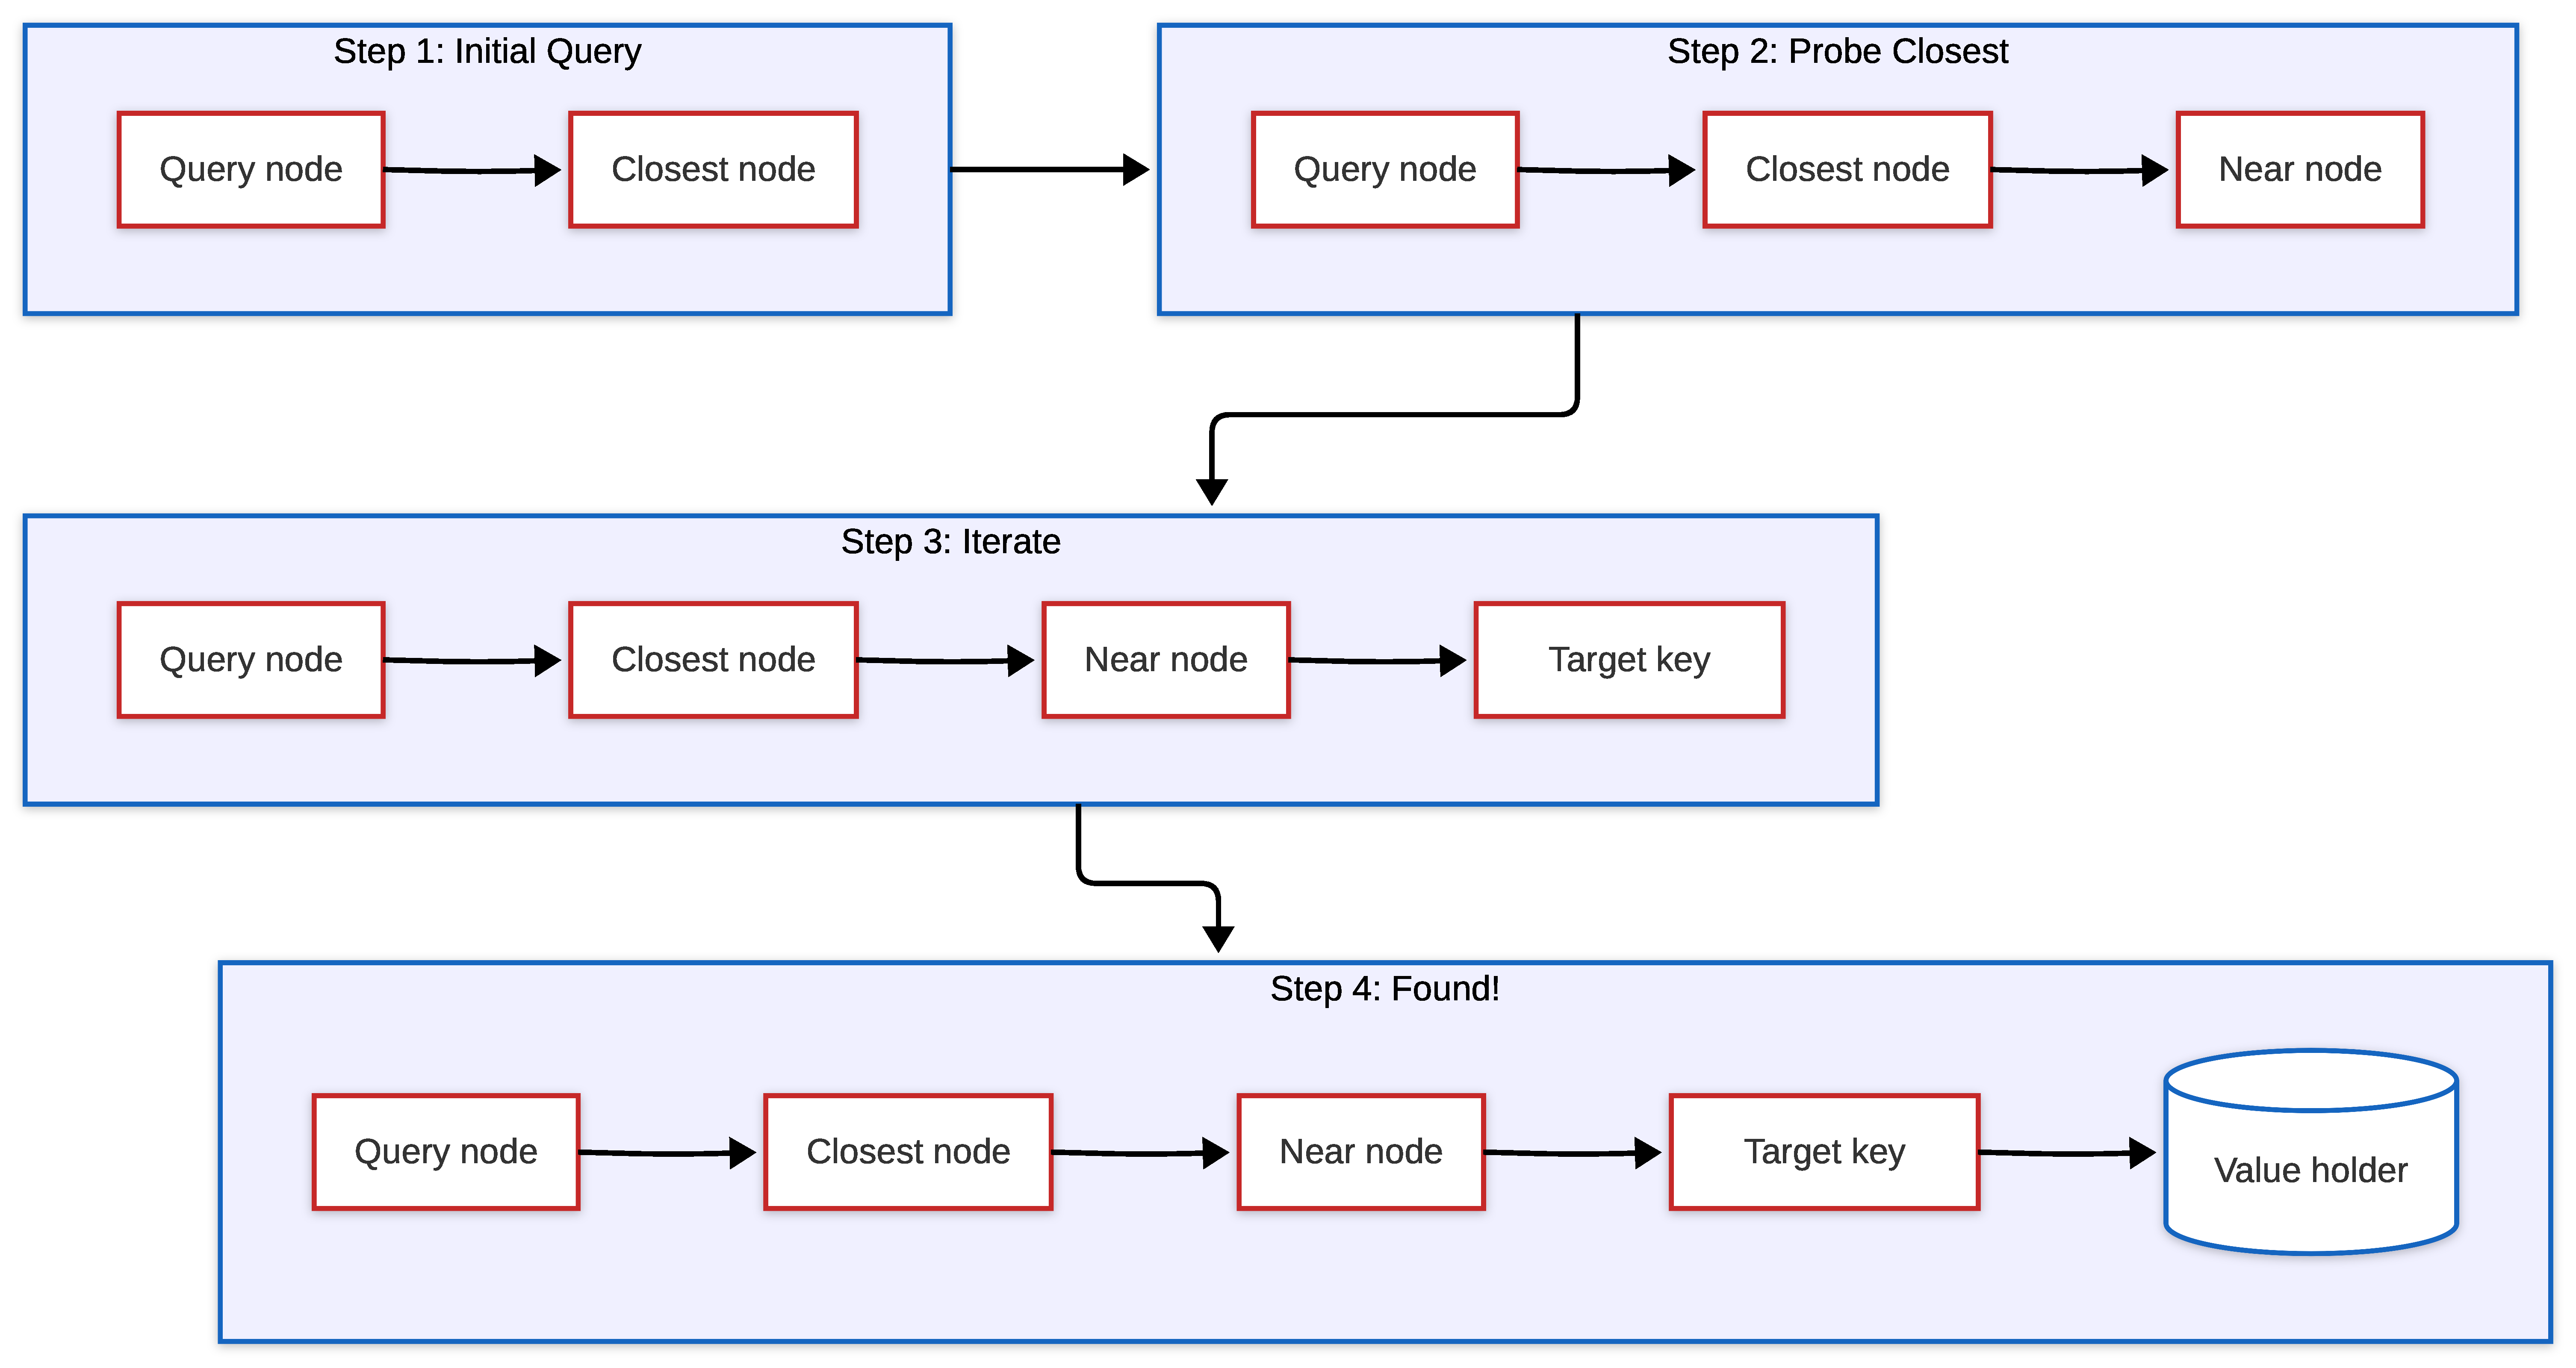
\includegraphics[width=0.75\linewidth]{figures/fig_p2p_dht_lookup.pdf}
  \caption{Kademlia DHT $O(\log N)$ lookup (own figure): a querying node routes through
    a sequence of intermediate nodes, each closer to the target key in XOR
    distance, until the value-holding node is reached \cite{MaymounkovKademlia2002}.
    Applied to adapter
    discovery, adapter descriptors would be indexed as key-value entries
    allowing peers to locate task-specific modules without a central registry.}
  \label{fig:dht_lookup}
\end{figure}

The Kademlia DHT is a candidate infrastructure for adapter-level discovery. In principle, adapter descriptors could be indexed as key-value entries in a DHT, allowing peers to locate adapters without a central registry. Whether task capability descriptors are sufficiently structured for DHT-based retrieval — and how such an index would perform under realistic churn — are open questions that the existing P2P literature has not examined.

\noindent The decentralised-learning findings of this chapter are
consolidated, alongside the other four sub-questions, in the centralised
discussion in Section~\ref{sec:synthesis_gap:answers}.
